\chapter{Design of Slope}
\label{chap:design}

\TODO{one/two summarizing paragraphs}


\section{Design goals}

Slope aims to provide a migration mechanism to applications to allow them to
seamlessly move their data structures, and as a result, their corresponding
operations, across their instances.

The most important design goal of Slope is being pluggable in existing
applications which work with their data in a partitionable way. That means if
the system designer has already came up with a way to partition
application data and computation into units that can be run independently on a
single machine, the task of integrating Slope into the system to make its data
structures or more complex computation units migratable should be trivial.

To be more specific, we aim for zero modification to the internals of the
application and minimal addition to the API of the computation unit to
correctly define its behavior during its life cycle in Slope.

The migration delay which we define as the elapsed time since the start of the
migration of an object until it is successfully migrated is an important
performance metric in Slope. However, directly measuring this duration may fail
in reflecting how the migration process impacts the application. Some
applications may prioritize responsiveness and would trade off some of their
throughput during the migration process to keep their tail latencies low.
Similarly an application may choose the opposite or any scenario in the middle.
Therefore it makes more sense to define migration performance from the view
point of the application based on how \emph{its} performance metrics degrade
as a result of the migration. Therefore while there is value in keeping the
migration delay small, we prioritize maximizing the \emph{usefulness} of the
application in the distributed setting during the migration.

\begin{figure}[H]
\centering

\ensurepdffromsvg{design-goals-pluggable.drawio}
\includegraphics[width=0.5\textwidth]{design-goals-pluggable.drawio}
\caption{
    Figure shows how Slope allows the already partitioned units of
    data/computation to be migrated across machines. However a need for request
    routing between the machines is introduced. This along with similar issues
    will be discussed in \TODO{a future section}.
}
\label{fig:designgoalspluggable}
\end{figure}

\section{Platform}
\label{sec:platform}

Applications have to call into Slope for initiating and carrying on the
migration operations. Since Slope requires intimate access to the application
memory, we need to carefully define what applications are supported
before discussing API and interactions.

We have chosen C++ as the platform to implement Slope, mainly because we need
to directly access process memory and manage the way it is allocated and used.
Whether or not these limitations can be eliminated, for example by using Slope
as a service or like a sidecar process, as opposed to a library are future
research directions.

On the flip side, as a result of the Applications conforming to the C++
allocation model which is used throughout the language and the standard
template library, much of already existing C++ code can be quickly made
migratable through Slope. STL containers for example, can be made migratable as long as they are given Slope's allocator for their allocator type parameter.

\begin{figure}[H]
\begin{alltt}
// Declaration of std::vector in the STL
template<
    class T,
    \textbf{class Allocator = std::allocator<T>}
> class vector;

template<typename T>
using mig_vector = std::vector<T, slope::memory::Allocator<T>>;

\end{alltt}
\caption{
\texttt{mig\_vector<T>} wraps \texttt{std{::}vector<T, Allocator<T>>}, setting
its allocator type to one that Slope provides. Objects of type
\texttt{mig\_vector<T>} are migratable as a result. Similarly
}
\end{figure}





\begin{figure}[H]
\begin{alltt}
// Declaration of std::vector in the STL
template<
    class T,
    \textbf{class Allocator = std::allocator<T>}
> class vector;

template<typename T>
using mig_vector = std::vector<T, slope::memory::Allocator<T>>;

template<class T, class Allocator>
class UserDefinedType \{
  static inline Allocator allocator;
  std::vector<T, Allocator> vector_;
  T *ptr_;
 public:
  template<typename... Args>
  UserDefinedType(Args&&... args):
    ptr_(\textbf{new (allocator.allocate(1))} T(std::forward<Args>(args)...)) \{ \}
  // ...
\};

\end{alltt}
\caption{
Similar to the case with \texttt{std{::}vector<T, Allocator>},
\texttt{UserDefinedType<T, Allocator>} is also migratable since it can work
with a supplied allocator that conforms to C++ allocator named requirement.
Furthermore, notice how the user defined type passes the allocator type parameter
to a member \texttt{std{::}vector}, demonstrating composition-friendliness, a
useful behavior for the application developer.
}
\end{figure}

\TODO{introduce what we gain from the custom allocator: At any point in time,
we know this and that about each object. details are discussed in forward ref
implementation section}
\TODO{We track all memory the object allocates + figure which shows the memory
of the object and what it points to all fall in the migratable memory}

\section{Architecture}
In coarse granularity, Slope consists of a control plane, a data plane,
a specialized distributed memory management
scheme/implementation, and a migration protocol
built on top
of the above. We have implemented the control plane and the data plane using
RDMA over infiniband because of how well the benefits of RDMA networking
fit our problem specifications, but the APIs which the two
sub-systems expose are not dependent on how RDMA works or how their internals
are implemented.

\subsection{Local memory layout}
Before we can discuss the main components of Slope, we need to discuss how
memory is managed in each application instance which uses Slope. Similar to
how this is done in \cite{memon2018ramp}, each program instance reserves a
large \TODO{elaborate how large is practical and why. Required for a future section} (e.g. equal to the machine's physical memory size) continuous part
of its virtual memory address space, starting at the same virtual address
on every machine, to be used by Slope using \texttt{mmap}.
This is done in program construction
time (i.e. before \texttt{main()}) and we will call this section of the virtual
address space the migratable memory or Slope memory. Note that mappings for
these pages are not yet generated and therefore the size of the slope memory
region can be expanded to the whole 64 bits of address on current machines.
We will manage the slope memory by 64KB page granularity which allows us to
leverage
the atomicity of \texttt{mprotect} in modifying the protections memory pages.
We do not use hugepages or contiguous physical memory as the former results in
loss of granularity and the latter needs to be done from inside the kernel and
typically at boot time before memory fragmentation gets in the way.

\begin{figure}
\centering
\ensurepdffromsvg{local-memory-management-phys-log.drawio}
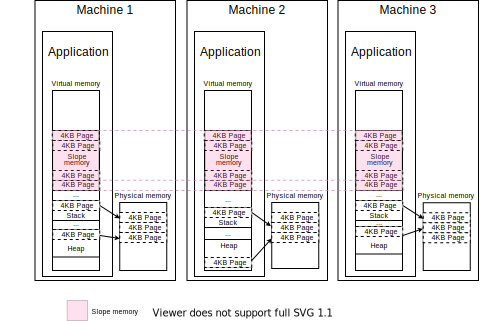
\includegraphics[width=1\textwidth]{local-memory-management-phys-log.drawio}
\caption{
    Placement of Slope memory within virtual memory address space on each node
    upon initialization.
    Notice how Slope memory is practically the \emph{same} on each node, as
    its size, starting address and therefore page boundaries are the same
    across all nodes. Also note how
    the 4KB pages from that region are not mapped to any physical memory pages
    yet.
}
\label{fig:localmemorymanagementphyslog}
\end{figure}

The way we lay Slope memory in the virtual address is central to how we later
discuss the migration process of an object. If an object was wholly contained
in the Slope memory region on Machine 1, meaning it had no references to memory
outside
of that region and no references to any resources to resources beyond the
scope of the application memory (E.g. a file descriptor), then if we moved all
of the memory belonging to that object to Machine 2, with the exception of
some house keeping tasks for example memory allocation and deallocation, the
object would continue to ``work'' in its new residence. This is the central
idea behind the migration of objects which is also used in \cite{memon2018ramp}
and all of the entities in Slope are desigend
to support the execution of this task in a seamless manner and improve its
performance.

It is important to note that although strict and inflexible, the requirement of
placing Slope memory on the same virtual address in all machines is,
unfortunately, a fundamental requirement. Figure \ref{localmemorymanagementfundamental}
shows an example of why this is the case. The implication is as long as the
application has any means of referencing the underlying virtual address of any
of its resources, its correct execution may end up depending on that address
staying the same at every point during the execution of the program. It would
be interesting to look into this issue and assess to what extent this can be
mitigated for example by allowing only ``named'' accesses to resources, similar
to how objects are accessed in Python (except the code boundary of calling into
external C functions). This way, we are effectively wrapping the application's
virtual address space in another layer of virtual addressing provided by the
language runtime.


\begin{figure}
\begin{alltt}

template<typename T> class ptr_hash;
template<typename T> class ptr_hash<T*> \{
  using Type = T*;
 public:
  size_t operator()(const Type& ptr) const \{
    return reinterpret_cast<std::uintptr_t>(ptr);
  \}
\};
int main() \{
  std::unordered_map<int*, int, ptr_hash<int*>> m;
  std::vector<int> v(0);
  // v.reserve(2); // Uncommenting will result in passing the assert
  v.push_back(1); m[&v[0]] = 1;
  v.push_back(2);
  assert(*(m.begin()->first) == m.begin()->second); // fails
\}

\end{alltt}
\caption{
    An example of reliance on a specific memory address. We create a hash
    function for pointers which simply uses their value, which is an address
    in virtual memory. The vector needs to move the contents of its underlying array to a
    bigger array before inserting the second element. At this point, from the viewpoint of
    \texttt{m}, \texttt{v} has ``moved'', effectively shifting its start
    address to a new virtual address. \texttt{m} has no way of figuring out
    the new address and no way of translating its address dependencies.
}
\label{localmemorymanagementfundamental}
\end{figure}


\subsection{Control plane}
Control plane provides an abstraction over which application instances can
execute migration operations and other side-tasks including distributed
memory management. For each operation that we support, we create a reliable
connected queue pair between each pair of machines, and pre-post to them
as many receive requests as we need to support concurrently. When a
machine pulls out a work completion from the completion queues assigned to
these queue pairs, a receive buffer is reposted to the corresponding queue to
make up for any other incoming requests, and a request flow starts during which
the two machines will go back and forth to carry out the operation. Although
the control plane can be practically replaced by any rpc framework, we do not
have much to gain from using \cite{kalia2016designguidelines} or
\cite{kalia2016fasst}, as the performance metrics in Slope are dominated mostly
by the performance of the data plane.

When using connected queue pairs, meta-data
from each queue has to exist on the device cache for any operations to be
carried out through that queue pair. As the number of queue pairs on each node
increases linearly with the number of nodes in the cluster when we connect the
QPs in a full-mesh manner, the performance of the application will collapse
after we pass a certain number of nodes in the cluster, which has
incentivized designs of RPC systems that use datagram queue pairs such as
\cite{kalia2019datacenter} and \cite{kalia2016fasst}, even though others such
as \cite{novakovic2019storm} have proposed hybrid one sided and two sided
schemes which scale well. We have not reached a point where we can directly
benefit from these optimizations as we are mostly throughput (data plane)
limited. Furthermore we use each queue pair repeatedly in short bursts after a
migration operation is triggered which avoids invalidating the ``active'' QP
meta-data from the cache during the migration. However the control plane
can be replaced entirely with any other RPC mechanism that achieves better
performance.

For co-ordination between machines (e.g. rendezvous protocol and transition
to ready to send state)
an out of band communication mechanism has to be used. We use memcached as
every node registers its queue pair and memory region parameters and
information and waits to receive the same information from its peers. This
phases only runs early in the program and does not have an effect on the
performance of they system after the initialization is finished, at which point
we can also take away the memcached server.

\subsection{Data plane}
The data plane is used to transfer the contents of a section of the Slope
memory to the same section in another node. As far as the data plane is
concerned, this is done in two major steps. Prefilling is done first, during
which the data plane will fill the corresponding addresses of the
Slope memory in a remote node from the same address in the current node, with
relaxed consistency requirements. Transfer operation follows shortly, during
which we ensure the contents of the above memory section in the source are
replicated to the same virtual addresses on the remote node. Prefilling is done
in 4KB page granularity, while transfer can be done in larger units, depending
on the continuity of the memory section that is being transferred.

Combining the above with other control mechanisms in the migration protocol, we
ensure that the data which underlies an object is correctly transferred to the
remote node after a migration. Optimistically, the transfer operation uses some
of the data that is already replicated to the remote node during the prefill
phase. Some of the prefilled data must be invalidated due to writes between the
prefill and the transfer phases. The participants need to correctly identify
the pages whose contents need to be invalidated to benefit from the performance
gain, while doing a correct transfer. This will be discussed in detail in section
\ref{sec:migrationprotocol}.

\subsection{Distributed memory management}

\subsection{Migration protocol}
\label{sec:migrationprotocol}
We observe the lifetime of a migratable data structure from the point it is
created uNTIL after we finish migrating it to another node. Throughout the
lifetime of the object and during the migration process, there are certain
conditions that need to be satisfied by the application for the migration
operation to finish correctly. As discussed later in this section,
in many of these cases, forcing the application to satisfy low level conditions
cannot be completely achieved by the library and the responsibility of
conforming to these conditions will be left to the application.

\subsubsection{Object creation}
A migratable object is created on the source machine. Let us call this object
the target object. Up until the point that
we initiate the migration, all of the memory allocations of the target object
must happen through
Slope's custom memory allocator through allocation contexts as discussed in
\ref{sec:platform}.
The application must satisfy the memory allocation requirements discussed in
\ref{subsec:trackallocations} to make sure Slope correctly keeps track of the
memory that each object references.

\subsubsection{Migration initiation}

\paragraph{Source}
initiates the migration by calling into Slope. From this point
on, the application instance on the source machine is neither allowed to
allocate more memory to the object by calling into the allocator using
an allocation context from this object, nor can it deallocate any memory that
this object references. This means the underlying memory of this object is now
fixed and read-only. The application can continue to read or write to the
Slope posts a send request to the QP that is shared
between the source and the destination machines, initiating the migration.
With this request, the source will include $n$ the number of continuous memory
chunks that the target object references.

\paragraph{Destination}
receives a migration request along with $n$, the number of chunks that need to
be transferred. The destination then populates another QP shared with the source
with with $n$ receive requests, each corresponding to one of the continuous
chunks of memory that underlies the target object. We switch to a different QP
to allow concurrent migrations to happen between pairs of nodes. The destination
then goes on to notify the source that it can receive the description of the $n$
continuous chunks. Why the destination will need to know about these before the
migration starts will become apparent during the next set of actions taken by
the destination.

\paragraph{Source}
receives the clear to send from the destination and sends the starting address
and the size of each of the $n$ chunks to destination.

\paragraph{Destination}
waits for $n$ chunk descriptions, and for each one of them, pins the
corresponding chunk in physical memory, so that the addresses that underlie the
target object can be used in RDMA read and write verbs. Notice how pinning the
whole slope memory to physical memory won't work as it will well exhaust the
available physical memory on each node. When the $n$ chunks are pinned
and are ready to be the target of the RDMA verbs, the destination responds back,
signaling that it has pinned all of the required chunks of memory.

\subsubsection{Prefill}

\subsubsection{Transfer}

\subsubsection{Post-transfer}

\subsubsection{Migration timeline at a glance}

\TODO{At the call to execute, the source is no longer allowed to write to the data structure and yields the ownership. Its reads will also return stale values.
  We cannot effectively mprotect away all of the memory that the data structure uses. A failed call will result in a SIGSEGV with no general way of
  recovering from it.}

\TODO{sequence diagram}

src: migrating n chunks
snk: send them

src: these are the n addrs
snk: pinned

src: prefill at address x, y, z, etc.
snk: got all prefills. Hand over the ownership

snk: locked, clear to read anything you want. x, y, z are dirty, and I'll also fill x for you
src: read y, z

\section{Implementation}
\TODO{incomplete}
We keep a thread local context stack which keeps track of the owner of each memory allocation. \TODO{Sequence diagram-like figure, denoting the ownership stack next to the function activation record stack of the thread}.

\subsection{keeping track of allocations}
\label{subsec:trackallocations}

\TODO{fill}
  procedures which allocate memory to or deallocate memory from the data structure. Typically all const qualified methods in c++ 
  are safe to be called after a call to prepare, however not every safe procedure is necessarily const qualified (e.g. updating an element in a vector)

fix the granularity by allocating to the same object from a page that it already owns.

\subsection{Multi-threading support}
Doesn't look fundamental since we are solving the problem cross node: theoretically run many instances.
One problem remains: how to co-ordinate memory deallocation. \TODO{fill}

- The ith machine owns the i/n'th section of the memory, assuming the machines have equal memory.
Machines use a two level memory
allocation scheme, in which they ask for large chunks (e.g. 4Gb) from other nodes in the cluster to make sure we do not exhaust
the address space that each node owns. This will eliminate the need for a centralized way of keeping track of object allocations.


Applications can bring their own memory allocator over the reserved regions of the shared address space that they have allocated: as long as they can call instead of mmaping a new memory themselves.
Deallocations return the memory to the owner of the big segment periodically, off the critical path. \TODO{These are tricky.. revisit}


\TODO{figure for per core and how threads interact with them}

\section{Computation model and API}

\TODO{fill}
Fundamentally every server has to be able to host an incoming object.
Since everything is async, this means that the object must know how to
"register" itself upon arrival in the remote node. Be it exposing a particular
api on a unix domain socket, or adding itself as an observer or worker to a blah.

each control plane has a fixed type

applications can intelligently use the time until ownership is transferred by
supporting read-only operations and even write operations with carefully
created static buffers that can contain unsupported (those that allocate/deallocate)
operations that the object has received after a call to initiate migration has
already been made.


\subsection{state machine}

\subsection{listen and serve}


\section{RDMA background}

discuss connection types

we use RC

discuss WR's and CQE's

discuss pinning

\section{Slope internals}

%  - Prefetch step happens in the prepare phase. source walks through the pages one by one, mprotects them to readonly, and
%    sends them to the corresponding addresses over RDMA.
%  
%    - This step is optional. If the data structure is under heavy usage and most of the memory is being touched, this
%    will only lengthen the migration process, during which the source cannot allocate/deallocate to the object that is being
%    migrated, without much improvement towards decreasing the handoff time, during which
%    none of the two machines have read or write access to the data structure.
%  
%  
%  ** Idea: From the call to execute, until when the source tells the sink about the call and send the
%  dirty pages that it needs to pull, we are losing time. What if the source pushes a few of the pages
%  based on a parameter that we optimize, to leverage the bandwidth during the idle time?
%   - I think regardless of the size of the data structure, this is a useful approach: If it's big,
%   only a small ratio is dirtied in between the phase changes and if it's small, then well, it's already small.
%   Since we can send 100Gb/s = 100Mb/ms, this is even close to the rate at which we dirty the pages, we win. \TODO{ This is not possible. The target memory is not
%   pinned before we tell them we're going to migrate into that specific part of their memory} \TODO{NO! this is happening after the prefill. The point here is to start the final transfer phase to make the handoff faster, not to make the whole migration process faster, which we don't really care that much about}
%   \TODO{How do we choose which pages to prefill? Can they express interest? Should we first send the mig_ptr
%   object headers to quickly generate the misses?}
%  
%  \section{Handling failures}
%  Migrations effectively allow us to persist a correct state of the data structure: We have a snapshot at migration time
%  
%  If a node goes away, we don't lose anything because of the point to point
%  nature of node communications. Every node knows who has allocated its memory
%  and can evict those leases if it desirable. No application fault tolerance
%  features provided aside from snapshots at migration time.
%  
%  
%  \section{Building systems on top of slope}
%  Discovery: can be done several ways: one way: lazy forwarding, keeping timestamps
%  of the migrations to figure out who knows the most recent information, 
%  Arp like protocol, 

% metric: change of (throughput per byte). What about the total time?
\TODO{Should this be in the evaluation section}
\TODO{Where should I raise the discussion about how these objects must be
used?}

\TODO{section: real world life-cycle of Slope and why it makes sense}
\TODO{discuss nested pointers, nested, recursive data structures}
